%%%%%%%%%%%%%%%%%%%%%%%%%%%%%%%%%%%%%%%%%%%%%%%%%%%%%%%%%%%%%%%
%
% Welcome to writeLaTeX --- just edit your LaTeX on the left,
% and we'll compile it for you on the right. If you give
% someone the link to this page, they can edit at the same
% time. See the help menu above for more info. Enjoy!
%
%%%%%%%%%%%%%%%%%%%%%%%%%%%%%%%%%%%%%%%%%%%%%%%%%%%%%%%%%%%%%%%

% --------------------------------------------------------------
% This is all preamble stuff that you don't have to worry about.
% Head down to where it says "Start here"
% --------------------------------------------------------------
 
\documentclass[12pt]{article}
 
\usepackage[margin=1in]{geometry}
\usepackage{amsmath,amsthm,amssymb}
\usepackage{tikz}
\usetikzlibrary{shapes,positioning}

\tikzset{ell/.style={ellipse,draw,minimum height=0.65cm,minimum width=1cm,inner sep=0.25cm}}

\usepackage{listings}
\usepackage{xcolor}

%New colors defined below
\definecolor{codegreen}{rgb}{0,0.6,0}
\definecolor{codegray}{rgb}{0.5,0.5,0.5}
\definecolor{codepurple}{rgb}{0.58,0,0.82}
\definecolor{backcolour}{rgb}{0.95,0.95,0.92}

%Code listing style named "mystyle"
\lstdefinestyle{mystyle}{
  backgroundcolor=\color{backcolour}, commentstyle=\color{codegreen},
  keywordstyle=\color{magenta},
  numberstyle=\tiny\color{codegray},
  stringstyle=\color{codepurple},
  basicstyle=\ttfamily\footnotesize,
  breakatwhitespace=false,         
  breaklines=true,                 
  captionpos=b,                    
  keepspaces=true,                 
  numbers=left,                    
  numbersep=5pt,                  
  showspaces=false,                
  showstringspaces=false,
  showtabs=false,                  
  tabsize=2
}

%"mystyle" code listing set
\lstset{style=mystyle}

 
\newcommand{\N}{\mathbb{N}}
\newcommand{\Z}{\mathbb{Z}}
 
\newenvironment{theorem}[2][Theorem]{\begin{trivlist}
\item[\hskip \labelsep {\bfseries #1}\hskip \labelsep {\bfseries #2.}]}{\end{trivlist}}
\newenvironment{lemma}[2][Lemma]{\begin{trivlist}
\item[\hskip \labelsep {\bfseries #1}\hskip \labelsep {\bfseries #2.}]}{\end{trivlist}}
\newenvironment{exercise}[2][Exercise]{\begin{trivlist}
\item[\hskip \labelsep {\bfseries #1}\hskip \labelsep {\bfseries #2.}]}{\end{trivlist}}
\newenvironment{problem}[2][Problem]{\begin{trivlist}
\item[\hskip \labelsep {\bfseries #1}\hskip \labelsep {\bfseries #2.}]}{\end{trivlist}}
\newenvironment{question}[2][Question]{\begin{trivlist}
\item[\hskip \labelsep {\bfseries #1}\hskip \labelsep {\bfseries #2.}]}{\end{trivlist}}
\newenvironment{corollary}[2][Corollary]{\begin{trivlist}
\item[\hskip \labelsep {\bfseries #1}\hskip \labelsep {\bfseries #2.}]}{\end{trivlist}}

\newenvironment{solution}{\begin{proof}[Solution]}{\end{proof}}
 
\begin{document}
 
% --------------------------------------------------------------
%                         Start here
% --------------------------------------------------------------
 
\title{Homework 1}%replace X with the appropriate number
\author{CSEN 4320 Computer Networks} %if necessary, replace with your course title
 
\maketitle
 
\begin{problem}{1} %You can use theorem, exercise, problem, or question here.  Modify x.yz to be whatever number you are proving
Briefly explain the following communication tasks:

i) routing\\
Routing is the process of choosing a path from the sender to the receiver, in a network of path options.
In the figure below, there are multiple different ways for node A to get to node F, and routing for example can choose
the path labeled with red numbers. This is important because sometimes certain paths might have high traffic and be congested so a different path will be better.\\
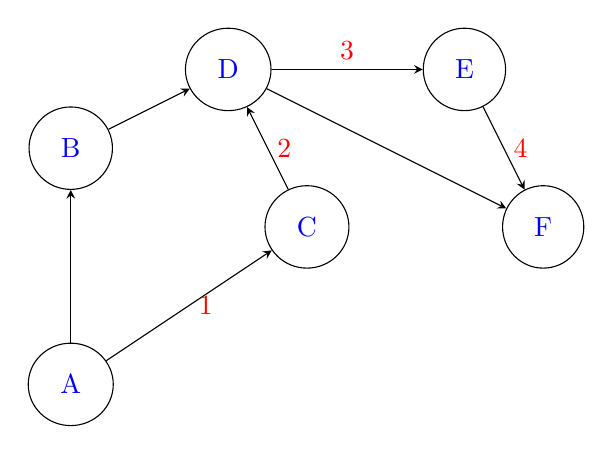
\begin{tikzpicture}[>=stealth]
    \node[ell] (a)at (0,0) {\color{blue}A};
    \node[ell] (b)at (0,3) {\color{blue}B};
    \node[ell] (c)at (3,2) {\color{blue}C};
    \node[ell] (d)at (2,4) {\color{blue}D};
    \node[ell] (e)at (5,4) {\color{blue}E};
    \node[ell] (f)at (6,2) {\color{blue}F};
    \draw [->] (a) to []node[right]{} (b);
    \draw [->] (a) to []node[right]{\color{red}1} (c);
    \draw [->] (c) to []node[right]{\color{red}2} (d);
    \draw [->] (b) to []node[right]{} (d);
    \draw [->] (d) to []node[above]{\color{red}3} (e);
    \draw [->] (d) to []node[above]{} (f);
    \draw [->] (e) to []node[right]{\color{red}4} (f);
\end{tikzpicture}

ii) flow control\\
Flow control is making sure that the amount of data sent by the sender is not more than the receiver can handle. 
This is important since if the sender sends more data than the receiver can process, then most of the extra data will be dropped and need to be sent again, wasting a lot of the effort.

iii) error detection\\
Since errors can occur during the transmission of data, error detection is finding out if such an error has happened so it can either be corrected, or the data can be resent.
\end{problem}

\begin{problem}{2}
Explain circuit switching and packet switching and mention one application for each of them.

Circuit switching is where once a path has been determined by the router for communication between sender and receiver, that path becomes fixed for the duration of the communication.
One application that uses circuit switching is the landline telephone network.

Packet switching is where the communication data is broken up into packets, where each packet can be routed differently between the sender and receiver, so there is no dedicated path.
One application that uses packet switching is the internet.
\end{problem} 

\begin{problem}{3}
What is the main reason for using the sequence number in a TCP header?

Since the data is split into packets that might arrive in a different order to the receiver, the sequence number tells the receiver the original order of the data in order to recombine the packets.
\end{problem}

\begin{problem}{4}
How many bits are there for the ``header length" field in the TCP header? Calculate the maximum possible size of the TCP header in octets.

There are 4 bits for the ``header length" field in the TCP header. The maximum value of this field is 15 units, where each unit is 4 octets, so 4*15=60 octets maximum.
\end{problem}

\begin{problem}{5}
What is the purpose of the ``Time to Live" field in an IPv4 header? Explain how it is used.

The purpose of the ``Time to Live'' field is to prevent packets that have been taking a long time to reach their destination from congesting the network. The way it is used is that it is set to some positive integer at the sender. Then for every router it goes to, the integer is checked and decremented by one.
If the integer becomes 0, then the packet is dropped rather than sent to the next router.
\end{problem}

% --------------------------------------------------------------
%     You don't have to mess with anything below this line.
% --------------------------------------------------------------
 
\end{document}